\documentclass[11pt,a4paper]{article}

\usepackage[utf8]{inputenc}
\usepackage[T1]{fontenc}
\usepackage[english]{babel}
\usepackage[a4paper,margin=2.4cm]{geometry}
\usepackage{graphicx}
\usepackage{float}
\usepackage{booktabs}
\usepackage{array}
\usepackage{xcolor}
\usepackage{tikz}
\usepackage{hyperref}
\usepackage{enumitem}
\usepackage{fancyhdr}
\usepackage{listings}
\usepackage{caption}

\usetikzlibrary{arrows.meta,positioning,shapes.geometric}

\pagestyle{fancy}
\fancyhf{}
\lhead{CSE344 - Homework \#5}
\rhead{Halit Batuhan ASLAN - 220104004003}
\rfoot{\thepage}

\setlist{nosep,leftmargin=18pt}
\hypersetup{colorlinks=true,linkcolor=black,urlcolor=blue}

\lstdefinestyle{bashstyle}{
    basicstyle=\ttfamily\small,
    frame=single,
    breaklines=true,
    backgroundcolor=\color{gray!8}
}

\newcommand{\screenshotbox}[2]{
    \begin{figure}[H]
        \centering
        \IfFileExists{#1}{
            \includegraphics[width=0.96\linewidth]{#1}
        }{
            \fbox{
                \begin{minipage}[c][6cm][c]{0.92\linewidth}
                    \centering
                    Add the uncut terminal screenshot here.\\[4pt]
                    Expected file: \texttt{\detokenize{#1}}
                \end{minipage}
            }
        }
        \caption{#2}
    \end{figure}
}

\begin{document}

\begin{titlepage}
    \centering
    \vspace*{2cm}
    {\Large Gebze Technical University}\\[0.4cm]
    {\large Department of Computer Engineering}\\[1.8cm]
    \rule{\linewidth}{0.5pt}\\[0.4cm]
    {\huge\bfseries CSE344 - System Programming}\\[0.3cm]
    {\Large\bfseries Homework \#5 Report}\\[0.2cm]
    {\large Priority-Based Cargo Delivery Simulation}\\[0.4cm]
    \rule{\linewidth}{0.5pt}\\[1.8cm]
    {\large\textbf{Student:} Halit Batuhan ASLAN}\\[0.3cm]
    {\large\textbf{Student ID:} 220104004003}\\[0.3cm]
    {\large\textbf{Date:} May 2026}
    \vfill
\end{titlepage}

\tableofcontents
\newpage

\section{System Design}

The program implements a fixed-size courier pool. All valid orders are read from the input file at startup, inserted into a shared priority queue, and only then courier threads are created. No new courier thread is created while the shift is running.

Each courier repeatedly takes one order from the queue, delivers it by sleeping for the requested simulation time, updates statistics, and then returns to the queue. When the queue is empty and no active delivery remains, all couriers leave the loop and the main thread writes the final statistics file.

In the updated assignment, one simulation unit is 500 milliseconds. The implementation uses one shared constant for this conversion, so console durations, total delivery time, courier totals, and sleeping time are calculated with the same value.

\begin{figure}[H]
\centering
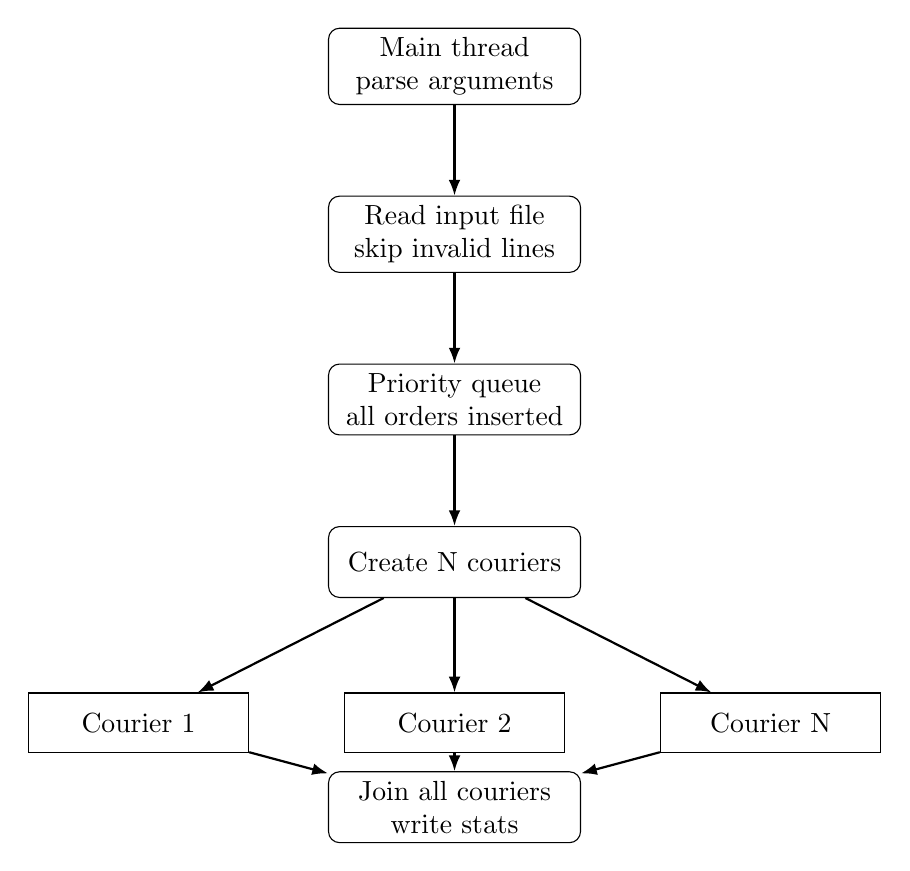
\begin{tikzpicture}[
    node distance=1.15cm,
    box/.style={rectangle,draw,rounded corners,align=center,minimum width=3.2cm,minimum height=0.9cm},
    smallbox/.style={rectangle,draw,align=center,minimum width=2.8cm,minimum height=0.75cm},
    arrow/.style={-{Latex[length=2mm]},thick}
]
\node[box] (main) {Main thread\\parse arguments};
\node[box,below=of main] (read) {Read input file\\skip invalid lines};
\node[box,below=of read] (queue) {Priority queue\\all orders inserted};
\node[box,below=of queue] (pool) {Create N couriers};
\node[smallbox,below left=1.2cm and 1.0cm of pool] (c1) {Courier 1};
\node[smallbox,below=1.2cm of pool] (c2) {Courier 2};
\node[smallbox,below right=1.2cm and 1.0cm of pool] (cn) {Courier N};
\node[box,below=2.2cm of pool] (join) {Join all couriers\\write stats};
\draw[arrow] (main) -- (read);
\draw[arrow] (read) -- (queue);
\draw[arrow] (queue) -- (pool);
\draw[arrow] (pool) -- (c1);
\draw[arrow] (pool) -- (c2);
\draw[arrow] (pool) -- (cn);
\draw[arrow] (c1) -- (join);
\draw[arrow] (c2) -- (join);
\draw[arrow] (cn) -- (join);
\end{tikzpicture}
\caption{General program flow}
\end{figure}

\subsection{Courier Lifecycle}

A courier starts in the depot, locks the queue mutex, and tries to pop the best available order. If it cannot work yet, it waits on the condition variable. After an order is taken, the courier releases the queue mutex before sleeping, so other couriers can continue to take work. At the end of a delivery, the courier updates atomic totals and its own local statistics.

\section{Priority Queue Design}

The priority queue is implemented as a binary min-heap. The comparison function first compares priority level and then order id. Since EXPRESS is represented with the smallest value, it naturally comes before STANDARD and ECONOMY. If two orders have the same priority, the lower id is placed earlier.

\begin{table}[H]
\centering
\begin{tabular}{lll}
\toprule
Priority & Internal value & Meaning\\
\midrule
EXPRESS & 1 & Highest priority\\
STANDARD & 2 & Normal priority\\
ECONOMY & 3 & Lowest priority\\
\bottomrule
\end{tabular}
\caption{Priority mapping}
\end{table}

The courier logs \texttt{DELIVERY\_START} immediately after popping the order while still holding the queue mutex. This keeps the visible start order consistent with the scheduling decision.

\section{Synchronization Strategy}

\begin{table}[H]
\centering
\begin{tabular}{p{4cm}p{9cm}}
\toprule
Primitive & Purpose\\
\midrule
\texttt{queue\_mutex} & Protects the priority queue, active delivery count, and shutdown flag.\\
\texttt{queue\_cond} & Blocks idle couriers and wakes them when the shift ends or shutdown starts.\\
\texttt{log\_mutex} & Protects every stdout line from interleaving.\\
\texttt{\_Atomic} counters & Tracks completed orders, cancelled orders, and total delivery time without a mutex.\\
\bottomrule
\end{tabular}
\caption{Synchronization primitives}
\end{table}

There is no busy waiting. Couriers use \texttt{pthread\_cond\_wait()} when they need to wait. The main thread uses a timed condition wait only to notice the SIGINT flag without doing unsafe work inside the signal handler.

\section{SIGINT Handling}

The signal handler only sets a \texttt{sig\_atomic\_t} flag. It does not print, lock a mutex, allocate memory, or cancel threads. The main thread observes this flag in normal control flow and performs the shutdown sequence.

\begin{enumerate}
    \item SIGINT arrives and the handler sets the flag.
    \item The main thread leaves its wait loop.
    \item The program enters shutdown mode under \texttt{queue\_mutex}.
    \item Pending orders are removed from the queue and logged as cancelled.
    \item Waiting couriers are awakened with \texttt{pthread\_cond\_broadcast()}.
    \item Couriers already delivering finish their current order.
    \item The main thread joins every courier and writes the final summary.
\end{enumerate}

\begin{figure}[H]
\centering
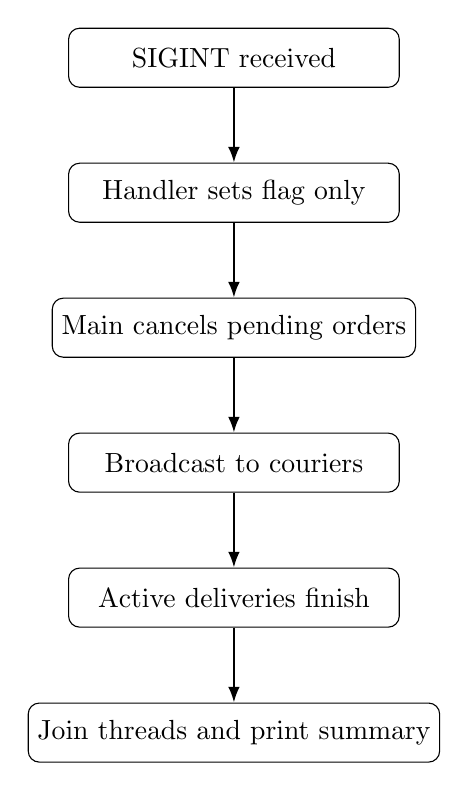
\begin{tikzpicture}[
    node distance=0.95cm,
    box/.style={rectangle,draw,rounded corners,align=center,minimum width=4.2cm,minimum height=0.75cm},
    arrow/.style={-{Latex[length=2mm]},thick}
]
\node[box] (sig) {SIGINT received};
\node[box,below=of sig] (flag) {Handler sets flag only};
\node[box,below=of flag] (cancel) {Main cancels pending orders};
\node[box,below=of cancel] (wake) {Broadcast to couriers};
\node[box,below=of wake] (finish) {Active deliveries finish};
\node[box,below=of finish] (end) {Join threads and print summary};
\draw[arrow] (sig) -- (flag);
\draw[arrow] (flag) -- (cancel);
\draw[arrow] (cancel) -- (wake);
\draw[arrow] (wake) -- (finish);
\draw[arrow] (finish) -- (end);
\end{tikzpicture}
\caption{SIGINT shutdown sequence}
\end{figure}

\section{Test Scenarios}

The following commands were used for the required scenarios. Each screenshot should show the complete terminal area from the command prompt to program exit.

\subsection{Scenario 1: Mixed 10 Orders}
\begin{lstlisting}[style=bashstyle]
./cargoGTU -n 3 -i 10orders_mix.txt -s stats.txt
\end{lstlisting}
This test checks that all 10 orders are completed and that \texttt{stats.txt} is written correctly. The updated homework removed the older requirement about all EXPRESS start lines appearing before the other priority classes in this scenario.
\screenshotbox{scenario1_10mixed.png}{Scenario 1 console output}

\subsection{Scenario 2: Economy Only}
\begin{lstlisting}[style=bashstyle]
./cargoGTU -n 10 -i 10orders_economy.txt -s stats.txt
\end{lstlisting}
This test checks the tie rule. Since all orders have the same priority, DELIVERY\_START lines must follow increasing id order.
\screenshotbox{scenario2_economyOnly.png}{Scenario 2 console output}

\subsection{Scenario 3: SIGINT}
\begin{lstlisting}[style=bashstyle]
./cargoGTU -n 2 -i 20orders_mix.txt -s stats.txt
# send Ctrl+C after about 2 seconds
\end{lstlisting}
This test checks that active deliveries finish, pending orders are cancelled, and completed plus cancelled equals the total number of valid orders.
\screenshotbox{scenario3_sigint.png}{Scenario 3 console output}

\subsection{Scenario 4: Valgrind}
\begin{lstlisting}[style=bashstyle]
valgrind --leak-check=full ./cargoGTU -n 3 -i 10orders_mix.txt -s stats.txt
\end{lstlisting}
This test checks memory cleanup. The expected result is zero errors and zero leaks.
\screenshotbox{scenario4_valgrind.png}{Scenario 4 Valgrind output}

\subsection{Scenario 5: High Concurrency}
\begin{lstlisting}[style=bashstyle]
./cargoGTU -n 10 -i 20orders_mix.txt -s stats.txt
\end{lstlisting}
This test is run multiple times. The completed count must stay the same, no order id should appear twice in DELIVERY\_START, and priority order must still be preserved.
\screenshotbox{scenario5_highConcurrency.png}{Scenario 5 console output}

\section{Challenges and Solutions}

\subsection{Keeping the visible order correct}

With several couriers, it is possible for one courier to pop an order and another courier to print first. To avoid that, the program prints \texttt{DELIVERY\_START} while the queue mutex is still held. The delivery itself starts after the mutex is released, so concurrency is not blocked for the delivery duration.

\subsection{Handling SIGINT safely}

Calling complex functions from a signal handler is unsafe in a multi-threaded program. The handler in this implementation only sets a flag. The main thread later cancels pending orders, wakes couriers, joins them, and writes the final files.

\subsection{Avoiding duplicate work}

Only one courier can pop from the priority queue at a time because the queue is protected by \texttt{queue\_mutex}. Once an order is removed, it no longer exists in the queue, so another courier cannot take the same order.

\section{Conclusion}

The implementation uses a fixed thread pool, a protected priority queue, condition variables for blocking, C11 atomic counters for shared statistics, and a clean shutdown path for SIGINT. The code is separated into small modules so parsing, scheduling, synchronization, logging, and statistics writing are easier to follow.

\end{document}
